El control de ejecución coordina la carga de programas, el inicio de las
sesiones y el avance del procesador. También determina qué ocurre cuando se
confirma una terminación, se solicita un reinicio o se vuelve a ejecutar una
imagen ya cargada. Para hacerlo, combina las órdenes recibidas desde la PC con
el estado de la sesión y las señales producidas por el pipeline.

\section{Reloj físico y ciclo efectivo}

Todo el sistema utiliza un reloj físico común, que sigue funcionando mientras
se carga un programa, se espera una orden o se transmite una respuesta de
Debug. La CPU, sin embargo, no necesariamente avanza en cada flanco: solo
realiza un \emph{ciclo efectivo} cuando el control activa
\code{cpu_cycle_fire}.

Un ciclo efectivo no equivale necesariamente a completar una instrucción. En
él, el pipeline puede avanzar normalmente, resolver una dependencia o un cambio
de flujo, confirmar \code{halt} o un fault, o completar trabajo durante el
drenado. Todos estos casos cuentan como ciclos de CPU.

Cuando \code{cpu_cycle_fire} está inactiva, la CPU permanece retenida, salvo
que una operación global, como reset, una carga aceptada o la preparación de
una sesión, modifique su estado. De esta manera, la actividad de UART y Debug
puede continuar sin agregar ciclos a la ejecución observada.

\section{FSM global de sesión}

La FSM global registra en qué fase se encuentra el sistema: por ejemplo, si
espera una imagen, prepara una sesión, ejecuta instrucciones o termina el
trabajo que queda en el pipeline. A partir de esa fase y de los eventos que
recibe, decide qué órdenes puede aceptar y cuándo autorizar un ciclo de CPU.

La FSM genera señales de control que utilizan el PC, el banco de registros,
las memorias y los demás bloques para actualizar su estado en el flanco
correspondiente. La implementación se distribuye entre \code{global_fsm.sv} y
\code{execution_control.sv}.

La tabla~\ref{tab:estados} presenta sus catorce estados. Para facilitar la
lectura de las transiciones, los diagramas que siguen muestran por separado la
carga, la ejecución y el drenado. Cada vista omite las permanencias sin eventos;
además, \code{RESET} tiene prioridad desde cualquier estado y una \code{LOAD}
aceptada prevalece sobre las transiciones locales.

\begin{table}[H]
  \centering
  \small
  \begin{tabularx}{\textwidth}{L{4.2cm}Y}
    \toprule
    \textbf{Estado} & \textbf{Significado} \\
    \midrule
    \code{NO_IMAGE} & No existe una imagen ejecutable confirmada. \\
    \code{LOADING} & Se recibe y valida una imagen nueva. \\
    \code{PREPARING_READY} & Se prepara la primera sesión de una imagen
    recién cargada. \\
    \code{READY} & Imagen y sesión preparadas, esperando \code{RUN} o
    \code{STEP}. \\
    \code{RUNNING} & Ejecución continua. \\
    \code{STEPPING} & Ejecución paso a paso, detenida entre comandos. \\
    \code{HALT_DRAIN_AUTO} & \code{halt} confirmado con trabajo anterior;
    drenado automático. \\
    \code{HALT_DRAIN_STEP} & \code{halt} confirmado; drenado mediante
    \code{STEP}. \\
    \code{FAULT_DRAIN_AUTO} & Fault confirmado con trabajo anterior; drenado
    automático. \\
    \code{FAULT_DRAIN_STEP} & Fault confirmado; drenado mediante \code{STEP}. \\
    \code{FINISHED} & Terminación normal con pipeline vacío. \\
    \code{FAULT} & Terminación excepcional con pipeline vacío. \\
    \code{PREPARING_RUN} & Preparación de una sesión nueva con \code{RUN}
    pendiente. \\
    \code{PREPARING_STEP} & Preparación de una sesión nueva con \code{STEP}
    pendiente. \\
    \bottomrule
  \end{tabularx}
  \caption{Estados de la FSM global.}
  \label{tab:estados}
\end{table}

Internamente, el estado se representa mediante catorce bits \emph{one-hot}:
cada estado tiene un bit asociado. Para Debug se genera, por separado, un código
externo de ocho bits. La tabla completa de transiciones y las señales de la FSM
se consultan en
\doc{architecture/session/execution_control.md}{Control de ejecución y sesión}.

La figura~\ref{fig:fsm-carga} muestra cómo se llega a una imagen disponible
para ejecutar. Después del reset, el sistema comienza en \code{NO_IMAGE}. Una
carga aceptada inicia la recepción en \code{LOADING}; si finaliza correctamente,
se prepara la primera sesión y se publica la imagen al entrar en \code{READY}.
Si la carga falla, el sistema vuelve a esperar una imagen válida.

\begin{figure}[H]
  \centering
  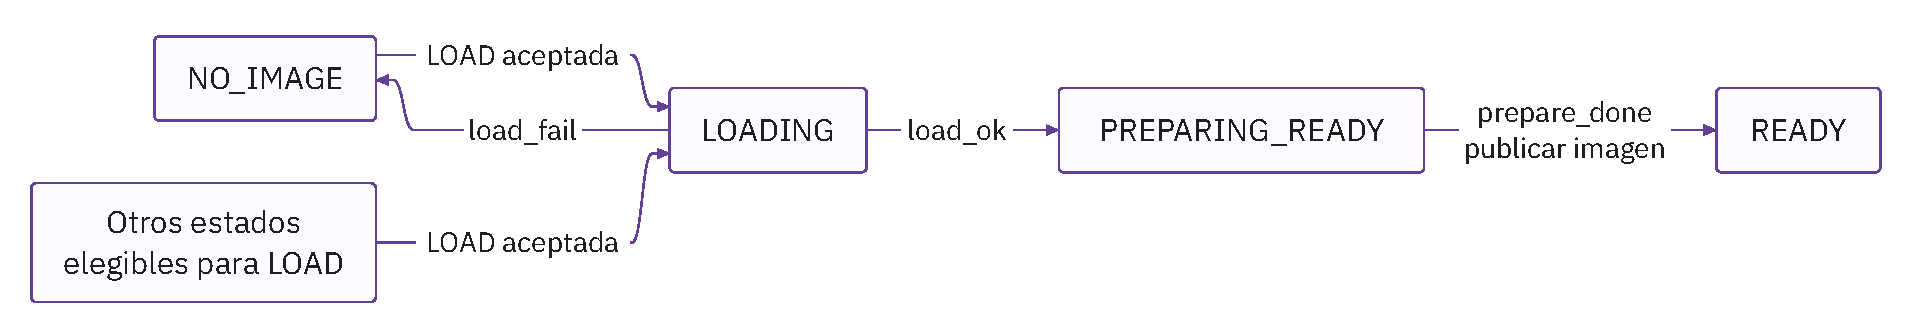
\includegraphics[width=0.94\textwidth]{fsm-carga.pdf}
  \caption{Carga y publicación de la imagen. Una carga fallida vuelve a
  \code{NO_IMAGE}; la preparación exitosa publica la imagen sin ejecutar CPU.}
  \label{fig:fsm-carga}
\end{figure}

\code{LOAD} es elegible en \code{NO_IMAGE}, \code{READY}, \code{STEPPING},
\code{HALT_DRAIN_STEP}, \code{FAULT_DRAIN_STEP}, \code{FINISHED} y
\code{FAULT}. Durante carga, preparación, ejecución continua o drenado
automático, una nueva solicitud de carga se rechaza y la actividad en curso
continúa según corresponda.

Una vez en \code{READY}, las órdenes \code{RUN} y \code{STEP} inician la
ejecución continua o paso a paso, respectivamente. La
figura~\ref{fig:fsm-ejecucion} también muestra qué sucede después de terminar:
la imagen puede reutilizarse, pero primero se prepara una sesión nueva para
que no herede el estado de la ejecución anterior.

\begin{figure}[H]
  \centering
  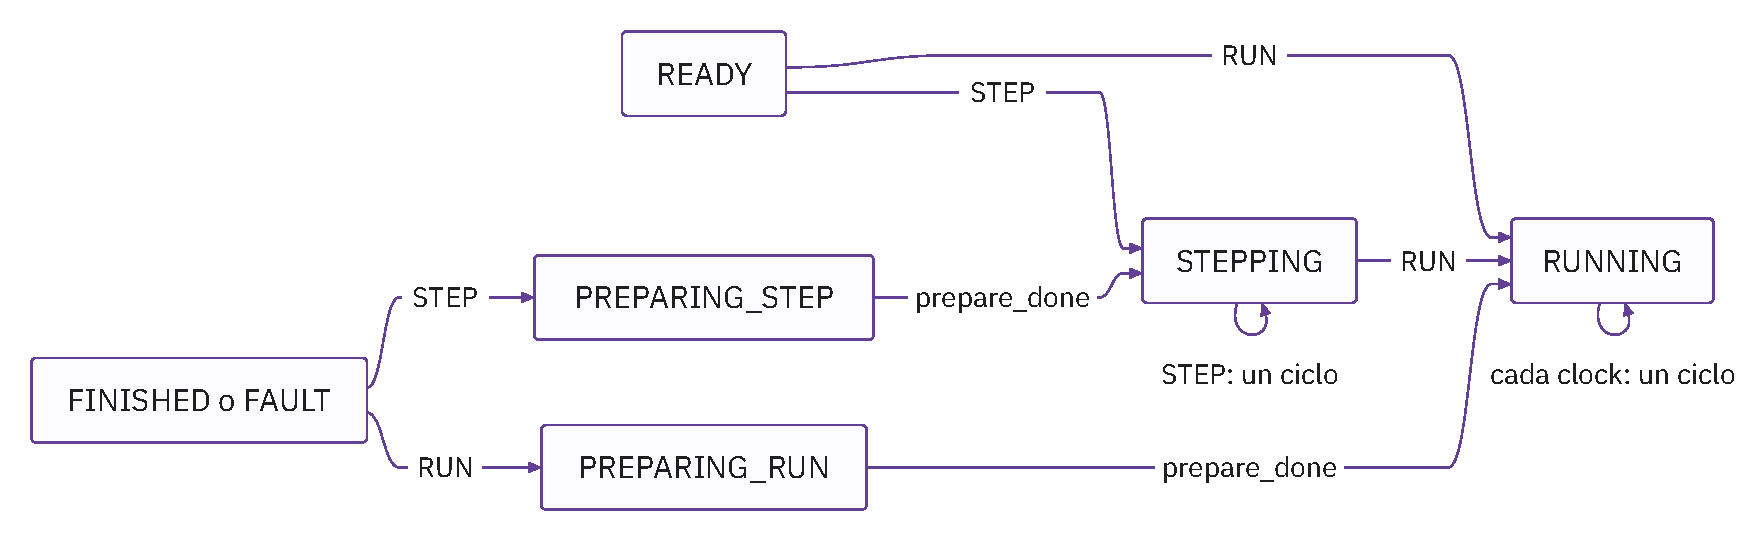
\includegraphics[width=\textwidth]{fsm-ejecucion.pdf}
  \caption{Inicio, reanudación y reutilización de una imagen. Las transiciones
  hacia \code{RUNNING} o \code{STEPPING} ejecutan el primer ciclo; desde un
  terminal, la orden espera a que termine la preparación.}
  \label{fig:fsm-ejecucion}
\end{figure}

Cuando se confirma \code{halt} o un fault, el pipeline puede conservar
instrucciones anteriores que deben completar sus efectos. La
figura~\ref{fig:fsm-drenado} muestra los estados que permiten terminar ese
trabajo. Si ya no queda ninguna instrucción anterior, el sistema pasa
directamente al estado terminal correspondiente.

\begin{figure}[H]
  \centering
  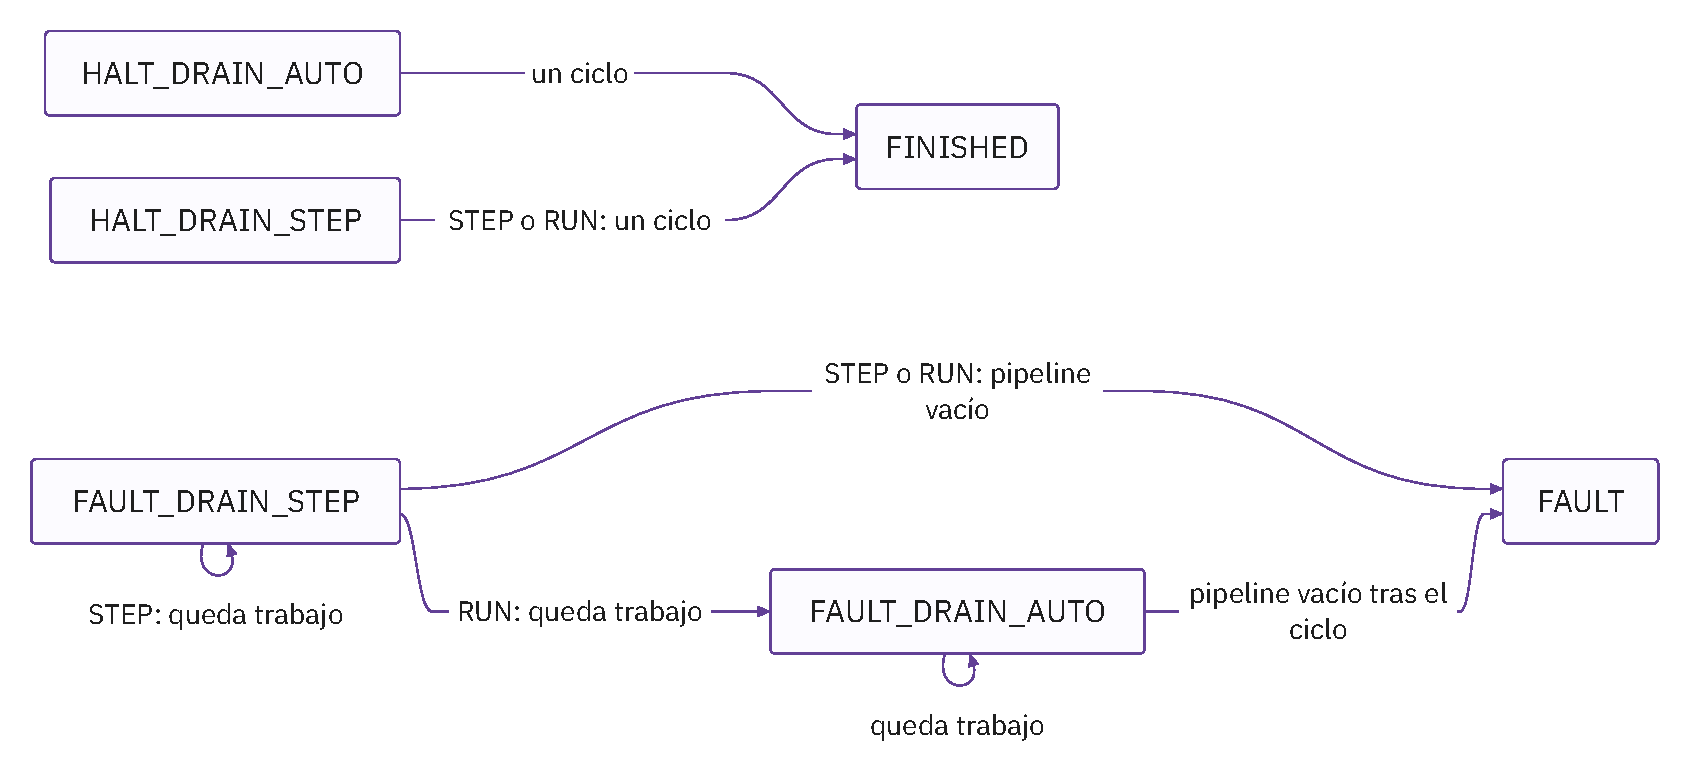
\includegraphics[width=\textwidth]{fsm-drenado.pdf}
  \caption{Drenado de instrucciones anteriores. El drenado por \code{halt}
  termina en un ciclo efectivo; el de fault puede requerir dos. En modo STEP,
  cada avance requiere autorización y RUN permite completar automáticamente.}
  \label{fig:fsm-drenado}
\end{figure}

\section{LOAD, RUN, STEP y RESET}

Las órdenes recibidas desde la PC permiten cargar una imagen y controlar su
ejecución. Cada una tiene un propósito diferente: \code{LOAD} incorpora un
programa, \code{RUN} y \code{STEP} determinan cómo avanza la CPU, y
\code{RESET} devuelve el sistema a su estado de reinicio.

\subsection{LOAD}

La carga comienza con una cabecera de seis bytes que contiene el código
\code{0x01} y el tamaño del programa, expresado como un entero sin signo de
cinco bytes en orden little-endian. La FPGA valida la solicitud antes de
aceptarla. Si es válida, responde \code{LOAD/ACCEPTED} y la PC envía los $N$
bytes anunciados. A medida que los recibe, el \code{Loader} forma palabras de
cuatro bytes y las escribe en IMEM.

Cuando se escribe la última palabra, \code{load_ok} indica que la recepción
terminó y la FSM pasa a \code{PREPARING_READY}. Allí se prepara el estado de
la primera sesión y, al finalizar, se publica la imagen y se responde
\code{LOAD/DONE}. La imagen anterior se invalida al aceptar la carga, por lo
que una transferencia parcial o fallida deja al sistema sin imagen ejecutable
hasta que se complete una carga posterior. El intercambio se detalla en
\doc{protocol.md}{Protocolo UART}.

\subsection{RUN}

\code{RUN} inicia o reanuda la ejecución continua. Si se acepta en
\code{READY}, el mismo flanco ejecuta el primer ciclo de la CPU, que realiza el
primer fetch con el pipeline vacío. A partir de entonces, en \code{RUNNING},
se solicitan ciclos automáticamente hasta que se confirme \code{halt} o un
fault.

La ejecución continua no implica ciclos idénticos: dentro de \code{RUNNING}
puede haber avance normal, stall \code{load-use}, redirect o confirmación de
\code{halt}/fault. Todos son ciclos efectivos. Un stall no detiene el modo
continuo; un redirect cambia el PC pero no abandona la sesión.

\subsection{STEP}

\code{STEP} permite observar la ejecución ciclo a ciclo. La CPU utiliza el
mismo datapath que en \code{RUN}, pero después de cada ciclo vuelve a esperar
una orden. Si se acepta en \code{READY}, el flanco de aceptación realiza el
primer fetch y la FSM pasa a \code{STEPPING}. Desde allí, otro \code{STEP}
autoriza un ciclo y \code{RUN} reanuda la ejecución continua.

Un paso corresponde a un ciclo de pipeline, no a la ejecución completa de una
instrucción. Por eso, en un mismo paso pueden avanzar varias instrucciones en
etapas diferentes.

Un stall \code{load-use} consume el \code{STEP}. Aunque el consumidor quede
retenido, el ciclo existió: el load y las instrucciones anteriores avanzaron. No
se ejecuta un segundo ciclo automático para completar la dependencia. Esta
distinción entre \code{STEP} y \code{HOLD} es fundamental para la observación y
se resume en la tabla~\ref{tab:step-hold}.

\begin{table}[H]
  \centering
  \small
  \begin{tabular}{lcc}
    \toprule
    \textbf{Situación} & \code{cpu_cycle_fire} & \textbf{Efecto} \\
    \midrule
    Stall \code{load-use} & 1 & parte del pipeline avanza; se consume un
    \code{STEP} \\
    \code{HOLD} & 0 & no hay avance de CPU ni consumo de \code{STEP} \\
    \bottomrule
  \end{tabular}
  \caption{Diferencia entre stall y \code{HOLD}.}
  \label{tab:step-hold}
\end{table}

\subsection{RESET}

El reset interrumpe la actividad vigente y tiene prioridad sobre los demás
efectos funcionales. Puede solicitarse mediante UART o con el botón físico de
la placa. Para el comando UART, el sistema transmite primero la respuesta
\code{RESET/ACCEPTED} completa, incluido el bit de Stop del último byte, y
después registra la solicitud de reset global. El botón físico puede actuar en
cualquier momento.

Al finalizar el reset, el sistema queda en \code{NO_IMAGE}, con PC, banco de
registros, contador, registros interetapa y tamaño confirmado en su estado
inicial. La imagen anterior deja de ser ejecutable y la preparación posterior
establece el cero lógico de DMEM. La secuencia temporal y las fuentes de reset
se detallan en \doc{architecture/platform/reset_integration.md}{Integración
del reset}.

\section{Preparación de una sesión}

La preparación establece un estado inicial limpio antes de ejecutar una
imagen. Se utiliza tanto después de una carga como cuando se vuelve a ejecutar
una imagen que ya terminó una sesión. En este último caso, las instrucciones
permanecen en IMEM y se restablece el estado de ejecución.

En el primer flanco de preparación se inicializan el PC, el banco de registros,
los registros interetapa y el contador, a la vez que se limpia la primera marca
de validez de DMEM. Los flancos siguientes limpian las demás marcas, una por
ciclo de reloj. Al terminar el recorrido, \code{prepare_done} indica que el
estado inicial está listo.

La FSM conserva el motivo de la preparación mediante tres estados. Aunque los
tres usan el mismo mecanismo, al finalizar entregan el control de manera
distinta:

\begin{itemize}
  \item \code{PREPARING_READY} prepara la primera sesión de una imagen recién
    cargada. Al terminar, publica la imagen y pasa a \code{READY}, donde espera
    una orden.
  \item \code{PREPARING_RUN} prepara una nueva ejecución continua de la imagen
    conservada. Al terminar, autoriza el primer ciclo y pasa a \code{RUNNING}.
  \item \code{PREPARING_STEP} prepara una nueva ejecución paso a paso. Al
    terminar, autoriza el primer ciclo y pasa a \code{STEPPING}.
\end{itemize}

La preparación completa dura 2049 ciclos de reloj en \code{REFERENCE} y 1001
en \code{ALT_1000}. A \SI{50}{\mega\hertz}, ambas duraciones caben en el
presupuesto de \SI{1}{\milli\second} para la preparación posterior a una carga.
Esos ciclos de preparación no incrementan el contador de la CPU.

\section{Drenado y terminación}

Una sesión termina normalmente al confirmar \code{halt} y termina de forma
excepcional al confirmar un fault. En cualquiera de los dos casos pueden quedar
en MEM o WB instrucciones anteriores que todavía deben completar sus efectos.
El drenado permite que esas instrucciones terminen mientras impide el ingreso
de trabajo nuevo. La instrucción que produjo el fault se descarta, \code{halt}
se consume en EX y las instrucciones posteriores también se descartan.

Si la confirmación ocurrió durante \code{RUN}, los estados
\code{HALT_DRAIN_AUTO} y \code{FAULT_DRAIN_AUTO} autorizan los ciclos restantes
automáticamente. Si ocurrió durante \code{STEP}, se entra en el estado de
drenado paso a paso correspondiente y cada \code{STEP} autoriza un ciclo más.
También puede solicitarse \code{RUN} para completar el drenado de forma
automática.

El control examina los indicadores de validez que tendrán los cuatro registros
interetapa después del ciclo. Cuando ya no queda trabajo, pasa a
\code{FINISHED} para una terminación normal o a \code{FAULT} para una
excepcional. Así, el último ciclo útil puede llevar directamente al estado
terminal sin agregar un ciclo vacío.

\section{Contador de ciclos}

El contador \code{cycle_count} permite conocer cuántos ciclos efectivos de CPU
transcurrieron durante la sesión. Es un valor sin signo de 64 bits que se pone
en cero durante la preparación y se incrementa una vez cada vez que se activa
\code{cpu_cycle_fire}.

El conteo incluye avances normales, stalls, redirects, confirmaciones de
\code{halt} o fault y ciclos de drenado. En cambio, durante \code{HOLD}, la
carga, la transmisión por UART, Debug y la preparación pueden transcurrir
ciclos del reloj físico sin que el contador avance.

Si alcanza \code{0xffffffffffffffff}, el incremento siguiente lo lleva a cero
sin generar un fault ni cambiar el modo de ejecución. Su valor completo se
incluye en el snapshot para relacionar el estado observado con los ciclos de la
sesión y compararlo con una simulación.

\section{Programas que no alcanzan \code{halt}}

Un programa puede ejecutar un bucle sin llegar a \code{halt}. En modo
\code{RUN}, si las instrucciones y sus accesos siguen siendo válidos, la CPU
continúa ejecutando sin un límite automático de ciclos.

Si el flujo intenta buscar una instrucción fuera de la imagen cargada, se
confirma un fault de acceso a instrucción. La sesión termina entonces en
\code{FAULT}, una vez completado el drenado que corresponda. Del mismo modo,
una instrucción ilegal produce un fault en lugar de una terminación normal.

En modo \code{STEP}, la CPU permanece detenida entre órdenes, aunque el
programa no tenga fin. Para interrumpir un \code{RUN} que no termina se utiliza
\code{RESET} por UART o el botón físico. Ambos invalidan la imagen y dejan el
sistema listo para recibir otra carga. Si una herramienta agota su tiempo de
espera, ese evento solo informa que dejó de esperar una respuesta; no significa
que la CPU haya terminado. Esta política corresponde a
\doc{decisions/DEC-SYS-002.md}{la decisión sobre ausencia de STOP/HALT}.

\section{Reprogramación}

Una imagen nueva puede reemplazar a la anterior sobre la misma configuración de
FPGA. Al aceptar \code{LOAD}, el sistema abandona la sesión vigente e invalida
el tamaño confirmado de la imagen anterior. Después de recibir la nueva imagen,
la preparación establece el estado inicial antes de publicarla.

La tabla~\ref{tab:reprogramacion} resume cómo participa cada elemento en este
proceso. En particular, el contenido físico de las memorias puede conservar
datos anteriores, pero el tamaño confirmado y las marcas de validez determinan
qué contenido pertenece a la nueva sesión.

\begin{table}[H]
  \centering
  \small
  \begin{tabularx}{\textwidth}{L{3.2cm}Y}
    \toprule
    \textbf{Elemento} & \textbf{Política} \\
    \midrule
    PC & Vuelve a cero en la preparación. \\
    IMEM & Conserva el array físico; la nueva imagen se escribe palabra por
    palabra. El tamaño confirmado delimita lo ejecutable. \\
    DMEM & Conserva el array físico; la preparación limpia las marcas de
    validez y el contenido no escrito se observa como cero. \\
    Banco de registros & Se inicializa en cero lógico durante la preparación. \\
    Registros interetapa & Se invalidan; los campos residuales no producen
    efectos. \\
    Debug & LOAD solo se acepta después de completar la respuesta anterior.
    Un snapshot de la sesión previa no representa el estado de la nueva. \\
    Control & La FSM inicia la carga y, si termina correctamente, prepara y
    publica la nueva imagen. Si la carga falla, queda en \code{NO_IMAGE}. \\
    \bottomrule
  \end{tabularx}
  \caption{Política de reprogramación.}
  \label{tab:reprogramacion}
\end{table}
